\section{EVALUATION AND DISCUSSION}

In this section, we present our assessment of
\tool{}, emphasizing the accuracy of our static
analysis in detecting side channels. Our evaluation of
\tool{} included a thorough examination of a
carefully selected set of benchmarks, influenced by \cite{hans}, featuring
a diverse range of programs, from those with vulnerabilities to benign
ones. These benchmarks were specifically designed to reveal typical and
intricate patterns in secret-dependent control flow, providing a
comprehensive examination of \tool{}'s effectiveness. 

The benchmarks consist of C programs compiled using 'arm-none-eabi-gcc,' a
cross-compiler toolchain tailored for generating code targeting ARM
Cortex-M and Cortex-R processors without an operating system (bare-metal).
The compiler is configured with the '-mcpu=cortex-m23' option to generate
optimized binary for ARM Cortex-M23 architecture. Here, we provide a brief
overview of selected benchmark programs. 

 \begin{figure}
  \centering
  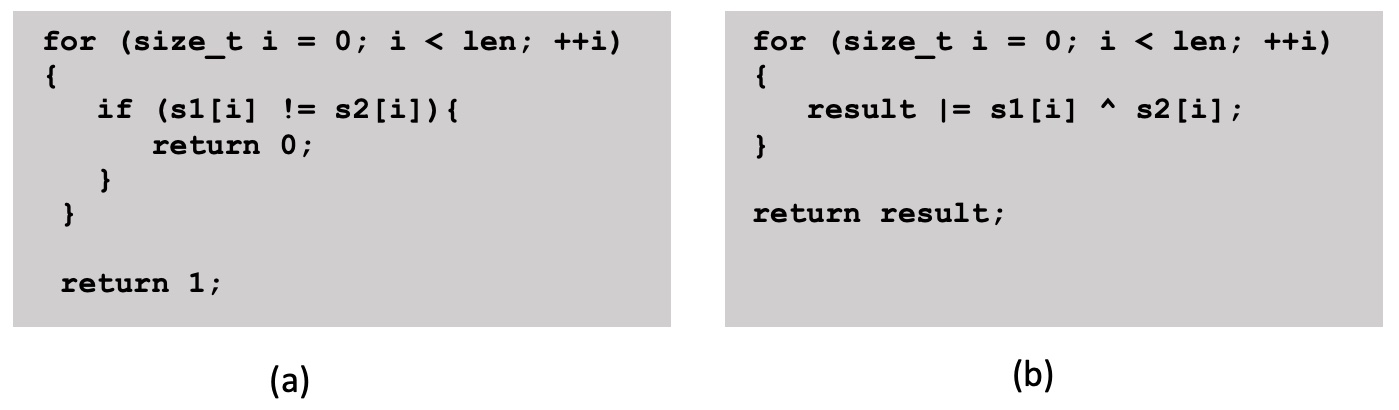
\includegraphics[width=\columnwidth]{figures/string.jpg}
  \caption{String Comparison}
  \label{fig:string}
\end{figure}


\begin{itemize}
%
    \item \textbf{busted:} This program features a vulnerability to the 'busted' attack, primarily due to a secret-dependent branching instruction. The vulnerability arises from the execution of the 'str' instruction at different time offsets within the 'then' and 'else' regions of the branch. However, it is free of start-to-end timing leaks due to having a balanced branch.
%
    \item \textbf{busted-free:} This program introduces dummy instructions, such as 'nop,' strategically placed in the code to delay the execution of the 'str' instruction in the 'else' branch by one clock cycle. This intentional delay ensures that memory access occurs at the same time offset. However, this approach results in an unbalanced branch.
%
    \item \textbf{strcmp:} This code performs a character-by-character comparison of two strings using a loop with an explicit branch. (refer to Fig. \ref{fig:string} (a)). However, because it relies on secret-dependent branches for the comparison process, it introduces potential timing side-channel vulnerabilities.
%
    \item \textbf{ constant\_time\_strcmp:} Utilizing a constant-time methodology, we enhance the string comparison code to resist timing side-channel attacks. This involves eliminating branches and employing mathematical formulas within the program (see Fig. \ref{fig:string} (b)). The comparison of characters is achieved through bitwise XOR (\textasciicircum) and bitwise OR ($|$) operations, eliminating the need for explicit branches and effectively mitigating timing side-channel vulnerabilities.
%
    \item \textbf{diamond:} This program features two branching instructions dependent on secret values and one independent branch.
%
    \item \textbf{loop:} The program contains a loop that relies on a condition with public data and includes a secret-dependent branch within the loop body. 
%    
    \item \textbf{secure\_loop:} In contrast, this code employs bitwise operations to eliminate the need for a conditional branch.
%    
    \item \textbf{multifork:} In this program, a switch statement evaluates the value of a secret variable and compares it against multiple cases. 
    
    \item \textbf{ifthenloop \& ifthenloop\_nop\_padded:} These programs
involve a branch dependent on secret data and a loop with a public variable
in its condition, executed if the branch is taken. In the
'ifthenloop\_nop\_padded' version, additional dummy instructions are
introduced to ensure a balanced execution across both branches.  
%    
    \item \textbf{ifthenlooplooptail:} This program introduces nested
secret-dependent branches and loops, creating a more intricate control flow
to thoroughly test \tool{}.
%
\end{itemize}


\begin{table*}
    \centering
		\caption{ Evaluation results for \tool{} on the benchmark
suite. For each compiled example program, we give an indication for C
program complexity (LOC = lines of code, CFG Size = number of nodes in the
program’s Control Flow Graph), execution time of
\tool{}, and list the vulnerabilities found by
\tool{}.}
  
		\label{tab:eval3}
  
		\begin{tabular}{llcccccc}
			\hline
			\textbf{Benchmark} &\textbf{LOC}
& \textbf{CFG}& \textbf{\ac{SCF}\textsuperscript{ARM}}& \textbf{Timing}& \textbf{Nemesis} &\textbf{BUSted} & \textbf{Storage}\\ 
		    {} &{} & \textbf{Size}& \textbf{exec time}& \textbf{Channel}& \textbf{Vulnerability} & \textbf{Vulnerability} & \textbf{Channel}\\ 
			\hline

busted & 14 & 20 & 3.042s & $\times$ & \checkmark & \checkmark & \checkmark \\ 

busted-free & 15 & 21 & 3.725s & \checkmark & \checkmark & $\times$ & \checkmark \\   

strcmp & 10 & 34 & 4.563s & \checkmark & \checkmark & \checkmark &      $\times$ \\ 

constant\_time\_strcmp & 13 & 39 & 2.564s & $\times$ & $\times$ &       $\times$ & $\times$ \\ 

diamond & 20 & 35 & 4.762s & \checkmark & \checkmark & \checkmark & \checkmark \\ 

loop & 16 & 49 & 3.330s & \checkmark &  \checkmark & \checkmark & \checkmark \\ 

secure\_loop & 22 & 58 & 4.902s & $\times$ & $\times$ & $\times$ & \checkmark \\ 

fork & 7 & 19 & 3.269s & \checkmark & \checkmark & \checkmark & \checkmark \\ 

fork\_nop\_padded & 12 & 24 & 3.769s & $\times$ & \checkmark & \checkmark & \checkmark \\ 

indirect & 20 & 29 & 3.460s & \checkmark & \checkmark & \checkmark & \checkmark \\ 

multifork & 15 & 34 & 4.013s & \checkmark & \checkmark & \checkmark & \checkmark \\

branchless\_multifork & 8 & 42 & 2.713s & $\times$ & $\times$ & $\times$ & \checkmark \\ 

ifcompound & 22 & 33 & 4.480s & \checkmark & \checkmark & \checkmark & \checkmark \\

call & 19 & 29 & 2.762s & $\times$ & $\times$  & $\times$ & \checkmark\\
		 		   
ifthenloop & 20 & 43 & 4.476s & \checkmark & \checkmark & \checkmark & $\times$ \\ 

ifthenloop\_nop\_padded & 25 & 50 & 4.608s & $\times$ & \checkmark & \checkmark & $\times$ \\

ifthenloopif & 28 & 74 & 6.890s & \checkmark & \checkmark & \checkmark & $\times$ \\ 

ifthenlooploop & 28 & 67 &  7.580s & \checkmark & \checkmark & \checkmark & $\times$ \\

ifthenlooplooptail & 38 & 110 & 8.136s & \checkmark & \checkmark & \checkmark & $\times$ \\

multiply & 5 & 12 & 3.789s & $\times$ & $\times$ & $\times$ & \checkmark \\
	   		   
		   \hline
		\end{tabular}
\end{table*}

In Table \ref{tab:eval3}, we present the experimental outcomes obtained by
applying \tool{} to the benchmark. Our results showcases that \tool{}
effectively analyzes intricate binaries designed for ARM Cortex-M23. The
tool not only adeptly identifies a spectrum of side-channel vulnerabilities
but also demonstrates its efficiency in swiftly and accurately detecting
sensitive data leakage. Keep in mind that utilizing branch balancing or
constant-time programming by itself cannot entirely eliminate the risk of
unintended information leakage within a program. In such instances, it
becomes imperative to take additional measures, such as securely storing
program outputs in a designated protected memory space or returning them in
an encrypted format.  These precautions provide an extra layer of security,
effectively mitigating the possibility of sensitive information being
unintentionally exposed to attackers, even when employing the mentioned
programming techniques.

\subsection{Discussion}

\paragraph{\textbf{Soundness}}
%
In this study, we emphasize the paramount importance of soundness in our
symbolic taint-tracking approach, aiming to establish credible security
assurances for Cortex-M23 programs. Central to our methodology is the
meticulous consideration of the execution time required for instructions on
a Cortex-M23 microcontroller. It is noteworthy that in the absence of
sophisticated architectural features such as paging, caches, or
out-of-order instruction pipelining, the time taken for instruction
execution is wholly deterministic.

The foundation of our proposed approach rests on the predictability of an
instruction's execution time, a characteristic intrinsic to Cortex-M23
microcontrollers. This inherent determinism serves as a cornerstone for the
soundness of our approach, enabling precise prediction of an instruction's
execution time. Consequently, programs certified by our \tool{} are
inherently fortified against timing-side-channel vulnerabilities.

\paragraph{\textbf{Nemesis Detection}}
%
As of our current knowledge, there have been no reported instances of a
Nemesis attack being executed on an ARM Cortex-M microcontroller.
Nevertheless, it is important to note that the ARM Cortex-M23 possesses all
the necessary prerequisites for a successful Nemesis attack. In general,
the Cortex-M23 processor tends to complete the current instruction before
handling an interrupt. This behavior, known as a "late-arriving interrupt"
model, means that if an interrupt is pending and becomes active during the
execution of an instruction, the processor finishes that instruction before
switching to the \ac{ISR}. However, the precise handling may vary depending
on the specific microcontroller implementation and the configuration of the
Nested Vectored Interrupt Controller (NVIC) that manages interrupts in the
Cortex-M series.

This interrupt handling mechanism introduces timing variations between
interrupted instructions, which could be leveraged by an attacker to
distinguish between secret-dependent branches. Furthermore, in our attacker
model, the adversary has the capability to control a timer device and
closely monitor \acp{ISR}, roughly resembling a configuration conducive to
launching a Busted attack \cite{busted}.

\paragraph{\textbf{Path explosion}}
%
Similar to other symbolic-execution tools, \tool{} encounters the widely
recognized challenge of state explosion, particularly evident when dealing
with larger binaries.  The exponential increase in path complexities
renders exhaustive exploration practically infeasible, potentially leaving
vulnerabilities undetected within unexplored paths.  Additionally, it is
noteworthy that Angr, the foundational symbolic execution framework for
\tool{}, introduces an inherent unsoundness by potentially concretizing
values during symbolic execution. These challenges are orthogonal to the
core contribution of this paper. Addressing the issue of path explosion and
enhancing the soundness of symbolic execution tools are recognized as
critical engineering tasks.  While beyond the scope of the current study,
we acknowledge them as essential aspects deserving of attention in future
work.


